\title{Assignment 1: CS 763}
\author{
  Sai Charith \\ 160050083
  \and
  Sanchit Jain\\ 160050043  
  \and
  Mayank Singhal\\ 160050039 
}

\documentclass[a4paper]{article}
\usepackage{amsmath}

\usepackage{amsfonts,amssymb,amsthm}
\usepackage[margin=0.94in]{geometry}
\usepackage{graphicx}
\begin{document}
\maketitle
%\makebox[\linewidth]{\rule{\paperwidth}{0.4pt}}
%\noindent\rule{12cm}{0.4pt}
\hrulefill
\\ \\
\textbf{Problem 3:} \\
The homogeneous coordinates of the given hyperbola in parametric form:
\[
A = 
\begin{bmatrix}
t \\
1/t \\
1
\end{bmatrix}
, t \neq 0 \]
\\  \\
Under the transform M,
\begin{equation*}
\begin{split}
& B = MA \\
\end{split}
\end{equation*}
\[
\implies
B =
\begin{bmatrix}
    0 & 0 & 1  \\
    0 & 1 & 0  \\
    1 & 0 & 0
    \end{bmatrix}
    \begin{bmatrix}
    t \\
    1/t \\
    1
    \end{bmatrix}
    , t \neq 0 
\]
\[
\implies
B = 
\begin{bmatrix}
1 \\ 
1/t \\
t
\end{bmatrix}
, t \neq 0
\]
\[
\implies
B = 
\begin{bmatrix}
1/t \\ 
1/t^2 \\
1
\end{bmatrix}
, t \neq 0
\]
\\
In geometric coordinates, B = $ (1/t, 1/t^2)$ , $ where $ $ t \neq 0 $ . \\
So, in geometric coordinates the image of hyperbola represents the parabola $ y = x^2. $  

\hrulefill\\ \\
\textbf{Problem 5a:} \\
Let R represent rotation, translation matrix and K represent camera internals and A be the direction of parallel linse passing through B and C. Any points on these lines can be represented as $P=tA+B$ , $Q=sA+C$ respectievely. So these points correspond to KRP and KRQ respectievely. Since R just rotates or transforms the lines still remain parallel. So RP and RQ correspond to $P' = t'A'+B'$ and $Q'=s'A'+C'$. Now as t' and s' tends to infinity, in the image they correspond to their respective vanishing points.\\
Therefore, 

\begin{equation*}
\begin{split}
& \;\;\;\qquad KP' = K(t'A'+B')\\
&\implies KP' = K(A'+\frac{B'}{t'}) \qquad (Homogenous\;\; Coordinates)\\ 
&\implies KP' = KA' \qquad (as \;\;t'\rightarrow\varpropto)\\
&\qquad \;\; KP' = KA' \qquad (Similarly\;\; for\;\; Q)\\
\end{split}
\end{equation*}
As, 
\[
K=
\begin{bmatrix}
    c       & cs & x_{H}  \\
    0       & c(1+m) & y_{H}  \\
    0       & 0 & 1
\end{bmatrix}
\]
the parallel lines vanish only if [0 0 1].A$'$ is not 0. (If it is 0 they vanish at infinity)\\ \\
\textbf{Problem 5b:}\\
Let ($x_1L+A_1$, $x_2L+A_2$), ($y_1M+B_1$, $y_2M+B_2$), ($z_1N+C_1$, $z_2N+C_2$) be the three sets of co-planer parallel lines after applying the R transformation.\\
Let K be the matrix representing internals of camera.\\
As the lines are coplaner $L.(M \times N) = 0 $  ie, where $L = [l_1,l_2,l_3]^T$, $M = [m_1,m_2,m_3]^T$, $N = [n_1,n_2,n_3]^T$
\[
Q=
\begin{bmatrix}
    l_1       & l_2 & l_3  \\
    m_1       & m_2 & m_3  \\
    n_1       & n_2 & n_3  \\
\end{bmatrix}
\]

\begin{equation*} 
\begin{split}
& det(Q) = 0 \\
\implies & det(Q^T)=0 \\
\implies & det(KQ^T)=0\\
\implies & det(K[L\; M\; N]) =0 \\
\implies & det([KL\;\; KM\;\; KN]) = 0\\
\implies & det([KL/a\;\; KM/b\;\; KN/c]) = 0 \qquad (Normalizing\;\; third \;\;coordinate)\\
\end{split}
\end{equation*}
$\implies$ area of triangle formed by KL, KM, KN (vanishing points) is zero. So the vanishing points of the three sets of coplaner parellel lines are collinear. 


\hrulefill\\


\textbf{\newline Problem 6:}

\begin{figure}[ht!]
 \centering
\caption{Picture with pixel values}
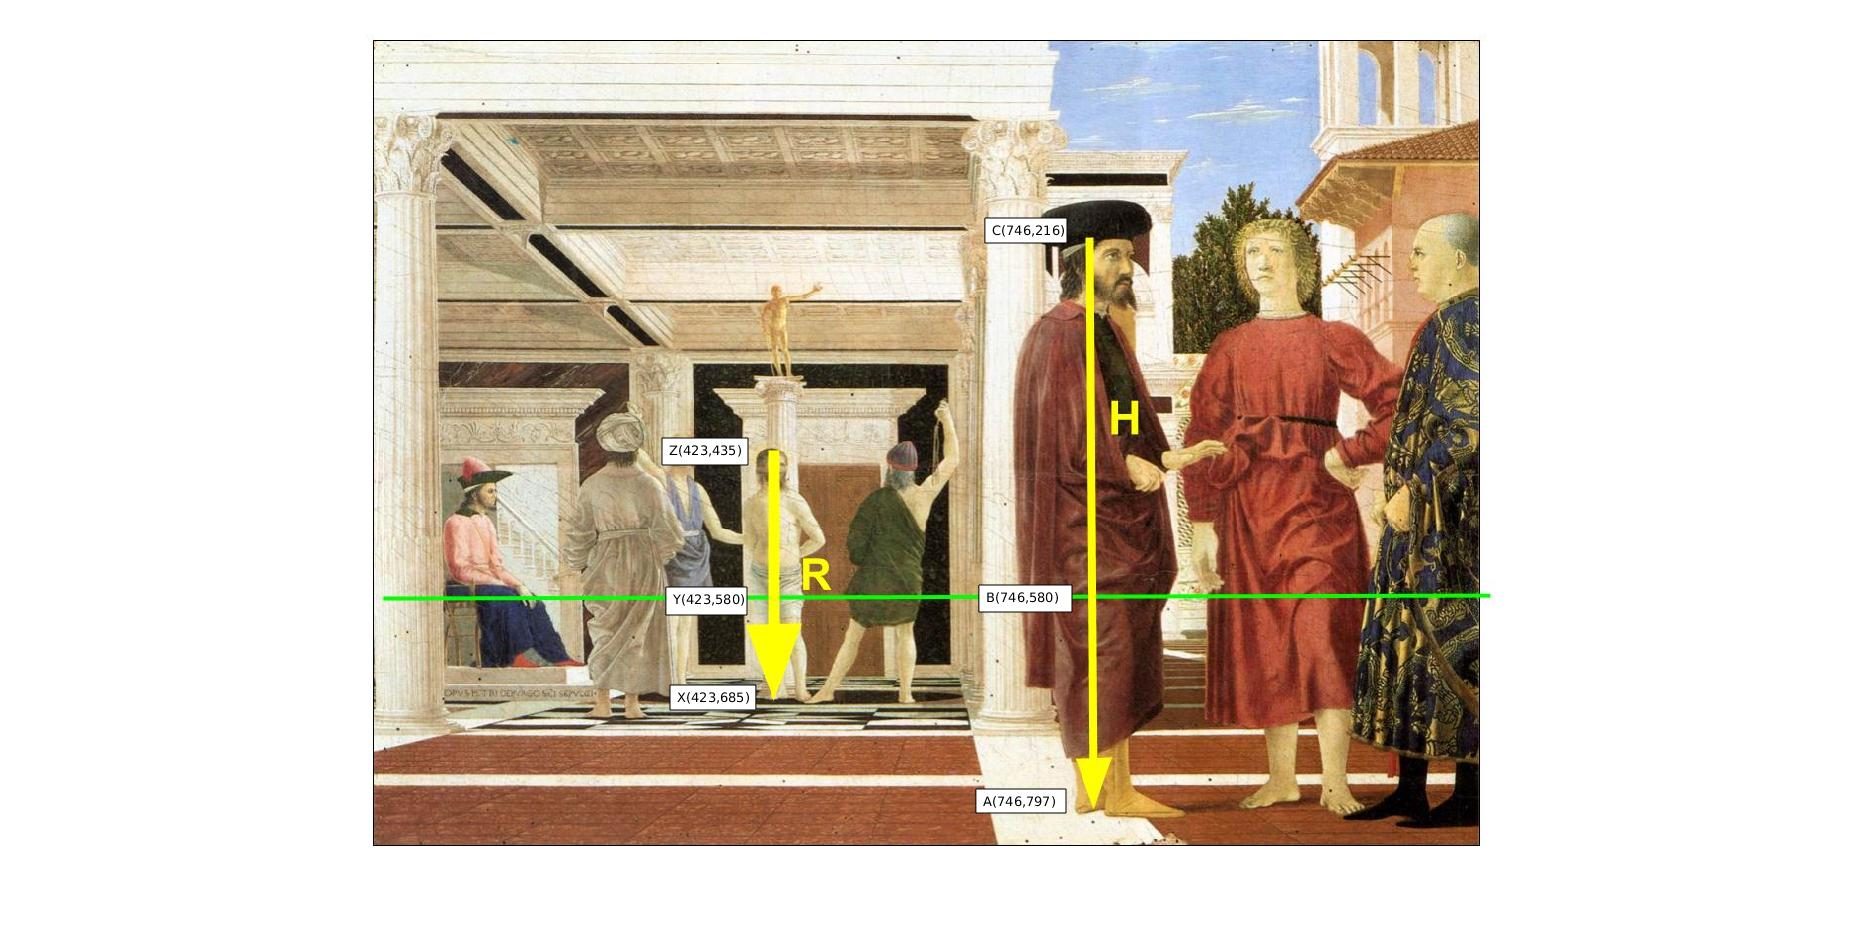
\includegraphics[width=1\textwidth]{Q6/measuredpicture.jpg}
\end{figure}

In the image the lines in y-direction do not vanish(as they are perpendicular to the axis of the image). So the line AC extended vanishes at infinity say at D. Similarly XZ vanishes at W. Let P' denote point P in world co-ordinates.

Using cross ratios we have

\begin{equation*} 
\begin{split}
 \frac{AC*BD}{AD*BC} &= \frac{A'C'*B'D'}{A'D'*B'C'} \\
\implies  \frac{AC}{BC} &=  \frac{A'C'}{B'C'} \\
\implies  \frac{AC-AB}{AC} &=  \frac{A'C'-A'B'}{A'C'} \\
\implies \frac{AB}{AC} &=  \frac{A'B'}{A'C'} \quad \textit{(equation 1)} \\
 \end{split}
\end{equation*}
Similarly
\begin{equation*} 
\begin{split}
 \frac{XZ*YW}{XW*YZ} &= \frac{X'Z'*Y'W'}{X'W'*Y'Z'} \\
\implies  \frac{XZ}{YZ} &=  \frac{X'Z'}{Y'Z'} \\
\implies  \frac{XY}{XZ} &=  \frac{X'Y'}{X'Z'} \quad \textit{(equation 2)}\\
 \end{split}
\end{equation*}
Now if we draw line passing through B and Y it coincides with horizon. This says that the line should be parallel to both sky and ground in the world co-ordinates. This says $ A'B' = X'Y' $ (Assuming both persons are on same horizontal level) . Now dividing the equations 1 and 2 we have
 
\begin{equation*}
\begin{split}
\frac{AB*XZ}{AC*XY} &= \frac{X'Z'}{A'C'} \\
\implies A'C' &= X'Z' \frac{AC*XY}{AB*XZ} \\
\end{split}
\end{equation*}
From the pixel values of the points we have  
\begin{equation*}
\begin{split}
A'C' &= 180\times\frac{(797-216)\times(685-580)}{(797-580)\times(685-435)} \\
\implies A'C' &= 202 cm
\end{split}
\end{equation*}
So, the hieght of the person in the image is 202 cm.


\hrulefill \\


\end{document}
